\chapter{Player stop reading}

Dear Players: You have finished reading. The next part contains adventures and surprises that I will not spoil. If you want to be a game master: continue.


\begin{figure}[!h]
    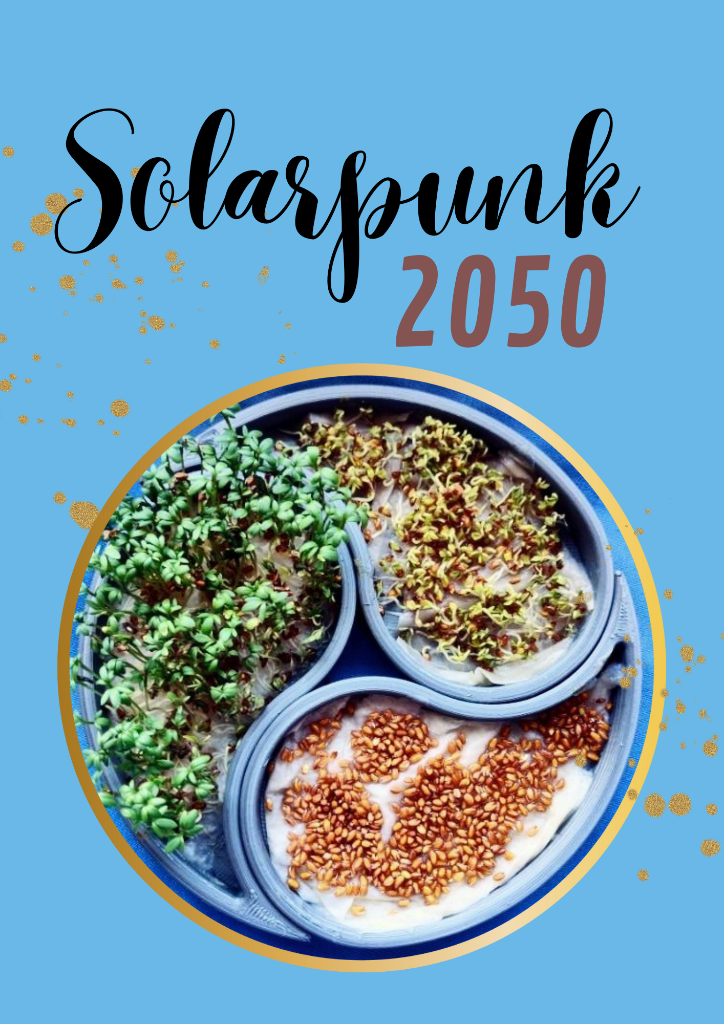
\includegraphics[width=\linewidth]{static/title.png}
    % \caption{A boat.}
    % \label{fig:boat1}
  \end{figure}

\section{Adventure structure}

There are a few tricks to give the adventure a solarpunk feel. A positive, inclusive, optimistic one.

\subsection{Protagonists}

The players are not the heroes, they are the protagonists. Many adventures are solved by using community resources.
Or by building a community first. Solving NPC problems and bringing them together and empowering them.

The "Die Hard" style hero will have a negative impact on the overall feeling.

\subsection{From the utopia}

Adventures begin in a solarpunk setting. A party, people building together.

\subsection{To a better utopia}

The end of the adventure should also be solarpunk: It can be a party, the construction of a new building for the community, a visit to some great places in nature... This is the reward for a successful adventure.

\subsection{Challenges}

There are challenges throughout the adventure. This setting has many of them. Choose one or two. Most of the time, the solarpunk utopia is not yet achieved when the protagonists enter the stage, or the utopia is out of balance. A backlash from the past (the "Dirty Road to Eden") can also cause trouble. Or friction between factions.

\subsection{A system is the baddie}

In many cases, it is not a single person or group of people who are the villains that need to be defeated to complete the mission. It is a system, a systematic injustice, or a situation caused by past failures that is the obstacle to be overcome.

\subsection{Solarpunk style solutions}

Building a community to help solve the problem is a Solarpunk-esque solution. Build things, fix things. Helping people. The quest should have some of these elements to make it feel Solarpunky.

\subsection{Topics}

Each quest should have several themes to explore. These could be
\begin{itemize}
    \item differences between the factions
    \item philosophies
    \item approaches to agriculture
    \item energy
    \item mistakes of the past
    \item dark secrets of the Dirty Road to Eden
\end{itemize}

As a GM, if you can get players talking after the game, you have done it right. In this game, there are no dragons to slay and brag about later. More important are the different points of view and approaches. Instead of the typical Dungeons and Dragons conversation on the bus to school "And then you threw a 20 and smashed the dragon's skull in", the solarpunk conversation should be more like "Well done for realising that their problem was caused by not switching to solar power 10 years ago and all the mess that decision caused. I'm glad you convinced them and showed them alternatives".